\chapter{Test-Time Augmentation and Ensembles}\label{ch:tta}

\section{Introduction}\label{sec:tta-why}
Averaging several noisy predictions is one of the oldest ideas in machine
learning~\citep{dietterich2000}. Suppose that each of $n$ predictions of some quantity has an error
with variance $\sigma^2$, and that every pair of errors has correlation $\rho$. The variance of
their average is then~\citep{hastie2009}
\begin{equation}
\operatorname{Var}\Big(\frac1n\sum_{v=1}^{n}\hat y_v\Big)
= \frac{\sigma^2}{n} + \frac{n-1}{n}\,\rho\,\sigma^2
= \sigma^2\Big(\rho + \frac{1-\rho}{n}\Big).
\label{eq:tta-variance}
\end{equation}
If the errors are independent ($\rho=0$), eight predictions reduce the variance eightfold. If they
are correlated, the variance of the average can never fall below $\rho\sigma^2$, however many
predictions we average. For example, with $\rho=0.9$, eight predictions remove less than a tenth of
the variance.

Equation~\eqref{eq:tta-variance} summarises most of this chapter. We tried two ways of obtaining
several predictions for the same photograph. \keyterm{Test-time augmentation}
(TTA)~\citep{krizhevsky2012} feeds a single model several transformed copies of the photograph, and
an \keyterm{ensemble}~\citep{lakshminarayanan2017} feeds the photograph to several models. Both help only to the extent that the errors of the individual predictions are
independent, and in our problem the errors turned out to be largely shared. In
Section~\ref{sec:tta-d4} we describe the transformations we used, and in Section~\ref{sec:tta-fusion}
the algorithm that combines instance masks from several views. Section~\ref{sec:tta-ensembles}
describes our ensembles of models, and Section~\ref{sec:tta-calibration} shows how to make the
confidence scores of different models comparable before combining them.
Section~\ref{sec:tta-m2f} applies test-time augmentation to the final model, and
Section~\ref{sec:tta-lesson} discusses what all these results say about the errors.

\section{The dihedral group}\label{sec:tta-d4}
The photographs have no preferred left or right, and a rotated image of the disk is still a
plausible image of the disk. Many astronomical images share this property, and \citet{dieleman2015}
exploited it in a network that classifies galaxies. The natural transformations are therefore the eight symmetries of a
square, which form the \keyterm{dihedral group} $D_4$: the four rotations by multiples of
$90^\circ$, each with or without a mirror reflection,
\begin{equation}
D_4 = \{\, r^k,\; f r^k \;:\; k = 0,1,2,3 \,\},
\end{equation}
where $r$ rotates the image by $90^\circ$ and $f$ reflects it from left to right. These
transformations move pixels without interpolating them, so no information is lost or invented,
unlike the rescaling of Section~\ref{sec:yolo-resolution}. Figure~\ref{fig:tta-d4} shows them
applied to a real filament.

\begin{figure}[t]
\centering
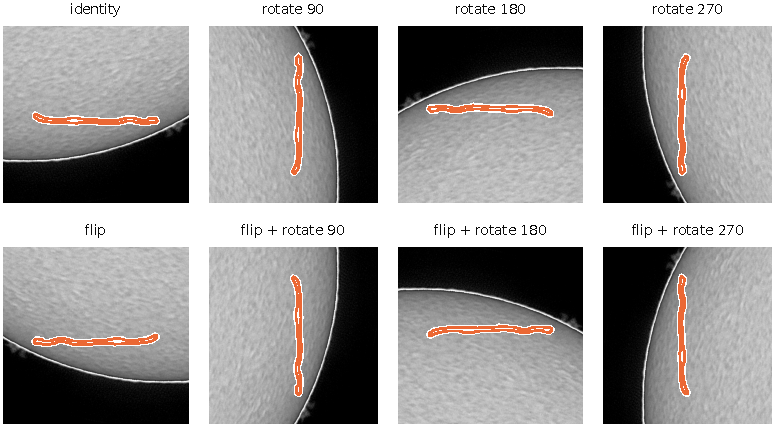
\includegraphics[width=\textwidth]{figures/fig_d4.pdf}
\caption{The eight dihedral views of one annotated filament, whose outline is drawn in orange. Each
view is a legitimate photograph of the same object, and a model sees each one slightly differently.
\generatedby{book/make\_book\_figures.py:fig\_d4}}
\label{fig:tta-d4}
\end{figure}

Test-time augmentation with $D_4$ runs the model once on each view and maps each predicted mask back
to the original orientation with the inverse transformation:
\begin{equation}
\mathcal{M}_g = \big\{\, g^{-1}(m) \;:\; m \in \mathrm{model}(g(\mathbf{x})) \,\big\},
\qquad g \in D_4 .
\end{equation}
If the model were exactly \keyterm{equivariant} to these transformations, meaning that
$\mathrm{model}(g(\mathbf{x})) = g(\mathrm{model}(\mathbf{x}))$ for every $g$, then all eight sets
$\mathcal{M}_g$ would be identical and TTA would change nothing. Convolutional networks are
equivariant to translations by construction, but not to rotations or reflections. Networks that
are equivariant to these transformations by construction exist~\citep{cohen2016}, but we did not use
one. Training with
flipped and rotated copies of the images makes them only approximately equivariant, and TTA exploits
the part of the equivariance that training did not achieve.

We also tried transformations of intensity. Applying a gamma curve to the photograph gave a PQ of
0.4294 at $\gamma=0.8$ and 0.4347 at $\gamma=1.2$, both below the 0.4411 obtained from the unchanged
image, so we dropped them.

\section{Fusing instances across views}\label{sec:tta-fusion}
For a semantic model, test-time augmentation is easy: we simply average the eight probability maps
pixel by pixel, as we did in exp004. For an instance model it requires a real algorithm, because
nothing tells us which mask in one view corresponds to which mask in another. One view may split a
filament that another view keeps whole, and each view has its own set of low-confidence extras. The
fusion rule in \file{experiments/exp\_033\_inference/src/cached\_tta.py} handles this greedily, in
the spirit of the weighted boxes fusion that detectors use~\citep{solovyev2021}, as described in
Algorithm~\ref{alg:tta-fuse} and Figure~\ref{fig:tta-fusion}.

\begin{algorithmblock}{Greedy fusion of instance masks across $N$ views\label{alg:tta-fuse}}
\item \textbf{input:} the scored masks of all $N$ views, mapped back to the original orientation; link threshold $\lambda=0.5$; vote fraction $\nu=0.5$
\item pool the masks of all views and sort them by decreasing score;
\item \textbf{while} some mask is unused \textbf{do}
\item \Ind take the most confident unused mask as the \emph{seed} of a new cluster;
\item \Ind add to the cluster every unused mask whose IoU with the seed is at least $\lambda$, and mark all members used;
\item \Ind fused mask $\leftarrow$ the pixels contained in at least $\max(1,\operatorname{round}(\nu n))$ of the cluster's $n$ members;
\item \Ind fused score $\leftarrow$ (mean score of the members) $\times\,\bigl(\tfrac12+\tfrac12\,n/N\bigr)$;
\item \Ind keep the fused mask if its area is at least 40 pixels;
\item \textbf{return} the fused masks and their scores
\end{algorithmblock}

The last factor in the fused score rewards \keyterm{support}, the share of the views that found the
object. A filament that all eight views found keeps its mean confidence, whereas a filament that
only one view found loses almost half of it.

\begin{figure}[t]
\centering
\begin{tikzpicture}[
  st/.style={box=#1, text width=1.95cm, minimum height=1.25cm, font=\sffamily\scriptsize,
             execute at begin node={\hyphenpenalty=10000}}]
  \node[st=inkmuted] (a) at (0,0) {predict on 8 views; map each mask back};
  \node[st=vizblue] (b) at (2.6,0) {pool all masks; sort by confidence};
  \node[st=vizblue] (c) at (5.2,0) {seed: best unused mask; members: IoU with seed $\ge 0.5$};
  \node[st=vizaqua] (d) at (7.8,0) {pixel vote: keep pixels in $\ge$ half of the members};
  \node[st=vizorange] (e) at (10.4,0) {score $=$ mean $\times\,(\frac12+\frac12\,n/N)$};
  \draw[flow] (a) -- (b); \draw[flow] (b) -- (c); \draw[flow] (c) -- (d); \draw[flow] (d) -- (e);
  \draw[flow] (e.south) -- ++(0,-0.45) -| node[note, pos=0.25, below=1pt] {repeat until every mask is used} (c.south);
\end{tikzpicture}
\caption{Instance fusion across test-time views. Clusters are seeded greedily in order of
confidence; each cluster's mask is a pixel vote among its members, and its score rewards support from
many views. \drawnin{book/chapters/ch08\_tta.tex}}
\label{fig:tta-fusion}
\end{figure}

The pixel vote in Algorithm~\ref{alg:tta-fuse} also controls the width of the fused mask.
Figure~\ref{fig:tta-vote} shows how the vote fraction affects a cluster of three overlapping member
masks. Requiring a vote from one member gives the union, which
grows the mask; requiring all members gives the intersection, which shrinks it; the majority vote
lies between the two. Recall from Section~\ref{sec:yolo-erosion} that the early YOLO masks were
already slightly too wide. The vote fraction therefore also acts as a control on the boundary, and a
later experiment (exp132) found that a stricter vote could replace the one-pixel erosion.

\begin{figure}[t]
\centering
\begin{tikzpicture}
  \foreach \px/\lab in {0/{at least 1 of 3: union}, 3.6/{at least 2 of 3: majority}, 7.2/{3 of 3: intersection}}{
    \node[note] at (\px,-0.85) {\lab};
  }
  % union
  \begin{scope}
    \fill[vizblue!45, rotate around={12:(0,0)}] (0,0) ellipse (1.0 and 0.33);
    \fill[vizblue!45, rotate around={4:(0.18,0.07)}] (0.18,0.07) ellipse (0.95 and 0.3);
    \fill[vizblue!45, rotate around={20:(-0.12,-0.04)}] (-0.12,-0.04) ellipse (1.05 and 0.28);
  \end{scope}
  % majority: union of the three pairwise intersections
  \begin{scope}[xshift=3.6cm]
    \begin{scope}
      \clip[rotate around={12:(0,0)}] (0,0) ellipse (1.0 and 0.33);
      \fill[vizblue!45, rotate around={4:(0.18,0.07)}] (0.18,0.07) ellipse (0.95 and 0.3);
      \fill[vizblue!45, rotate around={20:(-0.12,-0.04)}] (-0.12,-0.04) ellipse (1.05 and 0.28);
    \end{scope}
    \begin{scope}
      \clip[rotate around={4:(0.18,0.07)}] (0.18,0.07) ellipse (0.95 and 0.3);
      \fill[vizblue!45, rotate around={20:(-0.12,-0.04)}] (-0.12,-0.04) ellipse (1.05 and 0.28);
    \end{scope}
  \end{scope}
  % intersection
  \begin{scope}[xshift=7.2cm]
    \begin{scope}
      \clip[rotate around={12:(0,0)}] (0,0) ellipse (1.0 and 0.33);
      \clip[rotate around={4:(0.18,0.07)}] (0.18,0.07) ellipse (0.95 and 0.3);
      \fill[vizblue!45, rotate around={20:(-0.12,-0.04)}] (-0.12,-0.04) ellipse (1.05 and 0.28);
    \end{scope}
  \end{scope}
  % outlines of the three members in every panel
  \foreach \px in {0, 3.6, 7.2}{
    \begin{scope}[xshift=\px cm]
      \draw[vizorange, line width=0.6pt, rotate around={12:(0,0)}] (0,0) ellipse (1.0 and 0.33);
      \draw[vizaqua!80!black, line width=0.6pt, rotate around={4:(0.18,0.07)}] (0.18,0.07) ellipse (0.95 and 0.3);
      \draw[vizviolet, line width=0.6pt, rotate around={20:(-0.12,-0.04)}] (-0.12,-0.04) ellipse (1.05 and 0.28);
    \end{scope}
  }
\end{tikzpicture}
\caption{The pixel vote inside one cluster of three member masks, whose outlines are drawn in
colour. The region that is kept (blue) shrinks as the required share of members rises.
\drawnin{book/chapters/ch08\_tta.tex}}
\label{fig:tta-vote}
\end{figure}

\subsection{Voting on run-length encodings *}\label{sec:tta-ladder}
Our implementation performs the vote on run-length encodings, without ever decoding a mask into a
$2048\times2048$ array. It maintains a ladder of running regions, in which level $k$ holds the
pixels covered by at least $k$ of the masks seen so far. Each new mask $M$ updates the ladder from the
top down: level $k$ gains the pixels of level $k-1$ that $M$ also covers, and level 1 gains $M$
itself. After the last mask has been processed, the level equal to the required number of votes is
the answer. Listing~\ref{lst:tta-fuse} shows the ladder and the fusion loop.

\begin{lstlisting}[caption={Exact $k$-of-$n$ voting on RLE, and the greedy fusion. Condensed from
\file{experiments/exp\_033\_inference/src/cached\_tta.py} and
\file{experiments/exp\_097\_runpod\_yolo/src/evaluate\_ensemble.py}.},label=lst:tta-fuse]
def vote_rle(masks, needed):
    levels = [None] * needed          # levels[k-1]: pixels covered by >= k masks so far
    for i, mask in enumerate(masks):
        for k in range(min(i + 1, needed), 1, -1):          # top of the ladder first
            both = mu.merge([levels[k - 2], mask], intersect=True)
            levels[k - 1] = both if levels[k - 1] is None else mu.merge([levels[k - 1], both])
        levels[0] = mask if levels[0] is None else mu.merge([levels[0], mask])
    return levels[-1]

def fuse(entries, link=0.5, vote=0.5, sources=8):    # entries: (score, rle) from every view
    order = sorted(range(len(entries)), key=lambda i: -entries[i][0])
    rles = [e[1] for e in entries]
    ious = mu.iou(rles, rles, [0] * len(rles))          # pycocotools works on RLE directly
    used, output = set(), []
    for seed in order:
        if seed in used:
            continue
        used.add(seed)
        members = [seed] + [i for i in order if i not in used and ious[seed, i] >= link]
        used.update(members)
        binary = vote_rle([rles[i] for i in members], max(1, round(vote * len(members))))
        if mu.area(binary) < 40:
            continue
        score = float(np.mean([entries[i][0] for i in members]))
        output.append(dict(score=score * (0.5 + 0.5 * len(members) / sources), rle=binary))
    return output
\end{lstlisting}

\subsection{Example: the first attempt lost}\label{sec:tta-first}
Our first TTA experiment (exp007) used the same idea and \emph{lost}: the best of twelve fusion
settings scored 0.4035, against 0.4404 for a single view. At the time we identified two plausible
mechanisms, errors in the clustering and a vote that further eroded masks that had already been
trimmed, and we concluded that the result was a verdict on that particular implementation rather
than on TTA in general.

When we returned to the idea, we found a step that the first evaluation had skipped: it never
re-swept the confidence threshold after fusion. The support factor in Algorithm~\ref{alg:tta-fuse}
changes the scale of the scores. A filament found by every view keeps its mean confidence, whereas
one found by a single view loses almost half of it, so a threshold tuned for single-view scores is
wrong for fused scores. With the threshold swept again, the same fusion scored 0.4571 on validation.
A bootstrap over photographs (Section~\ref{sec:metric-uncertainty}, with 20,000 resamples) put the
gain at $+0.0166$, with a 95\% interval of $[+0.0039, +0.0303]$ and a probability of 0.995 that the
gain was positive. The fused model appeared on the leaderboard as 0.38, up from 0.36, and with the
emission threshold lowered to 0.35 it appeared as 0.39.

The general point is that any step that changes how scores are computed, such as fusion,
calibration, a support term or a new model, also moves the best operating point, so the confidence
threshold must be swept again after every such step. The grid of thresholds must also extend far
enough. The same problem appeared later, when a sweep started at 0.25 and the best fused rule lay at
the lower edge of the grid; we had to extend the grid down to 0.10.

\subsection{Variants that did not help}\label{sec:tta-variants}
Once the fusion worked, we tested its obvious variations, and none of them improved on it.
\begin{itemize}[leftmargin=*,itemsep=2pt]
\item \textbf{Soft voting.} Averaging the eight mask \emph{probabilities} before thresholding, instead
of voting on binary masks, scored at best 0.4569, against 0.4585 for the corresponding hard vote. It
found the same 841 true positives with six more false positives. Submitted as a probe, it appeared
on the leaderboard as 0.38.
\item \textbf{Mask non-maximum suppression.} Suppressing duplicates by the IoU of their masks rather
than of their boxes helped a single view (0.4453 against 0.4415), but it remained well below fusion,
and it appeared as 0.37.
\item \textbf{Other support scores.} Scoring clusters by the plain mean confidence of their members
(0.4466), or with a linear support term (0.4548), both lost to the rule of
Algorithm~\ref{alg:tta-fuse} (0.4571).
\item \textbf{Pruning by the number of views.} Removing clusters that fewer views supported always
reduced PQ. Most of the clusters that we kept were supported by all eight views, so agreement among
the views does not separate useful masks from harmful ones.
\end{itemize}

\section{Ensembles of models}\label{sec:tta-ensembles}
Fusing the predictions of \emph{different models} uses the same machinery with more sources. We built
ensembles of every kind we could, and Figure~\ref{fig:tta-ensembles} collects the results.

\begin{figure}[t]
\centering
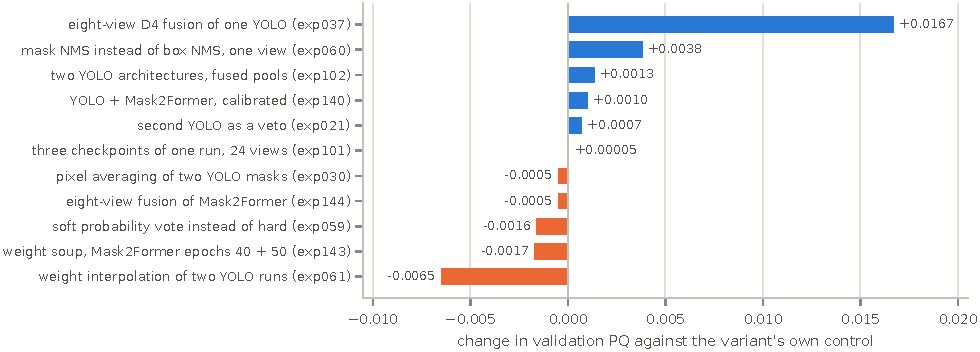
\includegraphics[width=\textwidth]{figures/fig_ensembles.pdf}
\caption{Every fusion, ensemble and weight-averaging variant we measured, shown as the change in
validation PQ relative to that variant's own control. Only the test-time fusion of the first YOLO
model moved the score by more than 0.004.
\generatedby{book/make\_book\_figures.py:fig\_ensembles}}
\label{fig:tta-ensembles}
\end{figure}

\paragraph{Two runs of the same architecture.} The models of exp002 and exp010 err in opposite
directions: the first gains recall at the cost of false positives, and the second gains precision at
the cost of misses. This looks like the textbook situation for an ensemble, but it did not work.
Their union scored 0.4124, requiring both models to agree scored 0.3740, and the best rule, which
used exp010 to veto the weaker masks of exp002, gained 0.0007 by removing 7 of 456 false positives.
The explanation lay in the errors themselves. Most of the false positives of exp002 were filaments
that the annotator of that record had not drawn, and exp010 saw the same filaments and predicted
them too. Averaging the two models' masks pixel by pixel (exp030) also lost. Of the 836 masks, 618
had a partner at an IoU of 0.5 in the other model, and the two models disagreed in the same places.

\paragraph{Checkpoints of one run.} In exp101 we pooled three checkpoints of the converged
YOLOv8l-seg run, with eight views each, for 24 views in all, and gained 0.00005. Checkpoints taken
from one training trajectory share almost all of their mistakes.

\paragraph{Averaging weights instead of predictions.} A \keyterm{model soup}~\citep{soups} averages
the weights of several models fine-tuned from the same starting point, and costs nothing at test
time.\footnote{Averaging weights tends to work when the models lie in the same basin of the loss
surface, as models fine-tuned from the same pretrained weights often do. \citet{soups} showed that
such averages can match or exceed the accuracy of the best individual model, and
\citet{izmailov2018} made a related observation for weights averaged along a single training
run.} Interpolating between exp002 and exp031 lost at every mixing weight (the best was 0.4349,
against 0.4415), and a soup of the Mask2Former's checkpoints from epochs 40 and 50 lost 0.0017 and
appeared on the leaderboard as 0.40, against 0.41 for epoch 40 alone.

\paragraph{Two YOLO architectures.} The first ensemble that helped at all combined models that
differed in more than their random seed: YOLO11m-seg trained at 1280 pixels and YOLOv8l-seg trained
at 2048. Each was first fused over its own eight views, and the two results were then fused with each
other. The ensemble gained 0.0013 and needed its own threshold sweep, because a mixed pool has a
different distribution of scores from either of its parents. As exp119, it appeared on the
leaderboard as 0.39, the same as its best member.

\section{Calibration: making scores comparable}\label{sec:tta-calibration}
Fusion averages the scores of the members of a cluster, which assumes that the scores mean the same
thing. For our models they did not. The best confidence threshold of the Mask2Former was 0.85,
whereas that of the YOLO models was 0.35, so averaging raw scores lets one model's scale dominate.
In exp140 we therefore \keyterm{calibrated}~\citep{guo2017} each source before fusing it, replacing each score by an
estimate of the probability that the metric cares about (Section~\ref{sec:recall-verifiers} explains
why the choice of this probability matters). We defined it as the fraction of a photograph's
annotation records that contain a filament matching the candidate with an IoU above 0.5.

The map from scores to probabilities should be monotone, since a higher score should never mean a
lower probability, but it need not be linear or sigmoidal. \keyterm{Isotonic
regression}~\citep{isotonic} fits exactly such a map. Given scores $s_i$ with labels $y_i$, it finds
the non-decreasing function $f$ that minimises
\begin{equation}
\sum_i \big(y_i - f(s_i)\big)^2 \quad\text{subject to}\quad s_i \le s_j \Rightarrow f(s_i)\le f(s_j).
\end{equation}
The \keyterm{pool-adjacent-violators} algorithm~\citep{ayer1955} solves this problem in a single pass over the sorted
scores (Algorithm~\ref{alg:tta-pav}). Each distinct score starts as its own block. Whenever a block's
mean label is lower than the mean of the block before it, the two blocks violate the monotonicity
constraint, so we merge them, and we keep merging backwards until the block means increase again.
The final block means are the fitted values.

\begin{algorithmblock}{Pool adjacent violators, for isotonic regression\label{alg:tta-pav}}
\item \textbf{input:} the distinct scores in increasing order, each with the sum and count of its labels
\item \textbf{for} each distinct score, in increasing order, \textbf{do}
\item \Ind push a new block containing that score's label sum and count onto a stack;
\item \Ind \textbf{while} the stack has at least two blocks and the mean of the second-last exceeds the mean of the last \textbf{do}
\item \Ind\Ind merge the last two blocks by adding their label sums and counts;
\item \textbf{return} the mean label of each block, as a step function of the score
\end{algorithmblock}

\begin{lstlisting}[caption={Isotonic calibration by pool-adjacent-violators. Condensed from
\file{experiments/exp\_140\_three\_way\_ensemble/src/ensemble.py}.},label=lst:tta-isotonic]
def isotonic_fit(scores, labels):
    values, inverse, counts = np.unique(scores, return_inverse=True, return_counts=True)
    sums = np.bincount(inverse, weights=labels)
    blocks = []                                   # [sum of labels, weight, sum of scores]
    for x, s, c in zip(values, sums, counts):
        blocks.append([s, float(c), x * c])
        while len(blocks) > 1 and blocks[-2][0] / blocks[-2][1] > blocks[-1][0] / blocks[-1][1]:
            s2, c2, sx2 = blocks.pop()            # a violation: pool with the block before
            blocks[-1][0] += s2; blocks[-1][1] += c2; blocks[-1][2] += sx2
    centres = np.array([b[2] / b[1] for b in blocks])
    means = np.array([b[0] / b[1] for b in blocks])
    return centres, means                         # apply with np.interp(score, centres, means)
\end{lstlisting}

We fitted the maps on the validation split. To obtain validation numbers that were not biased by
this fitting, we \keyterm{cross-fitted} them~\citep{chernozhukov2018}: we split the photographs into two folds and calibrated
the candidates of each fold with a map fitted on the other fold, so that no candidate was calibrated
using its own photograph. The fitted maps were informative in themselves. The Mask2Former turned out
to be over-confident in the middle of its range: a score of 0.854 corresponded to a 45\% chance of
matching a record, 0.94 to 64\%, and 0.97 to 88\%. The YOLO models were closer to being calibrated.
The results were as follows:
\begin{center}\footnotesize
\setlength{\tabcolsep}{4pt}
\begin{tabular}{@{}lccccc@{}}
\toprule
sources & scores & YOLO eroded & PQ & TP / FP / FN & threshold \\
\midrule
Mask2Former alone & raw & -- & 0.47052 & 881 / 361 / 444 & 0.85 \\
all three models & raw & no & 0.46677 & 859 / 342 / 466 & 0.50 \\
all three models & calibrated & no & 0.46719 & 877 / 372 / 448 & 0.35 \\
all three models & calibrated & yes & 0.46924 & 832 / 297 / 493 & 0.40 \\
YOLOv8l + Mask2Former & calibrated & yes & \textbf{0.47151} & 849 / 303 / 476 & 0.40 \\
\bottomrule
\end{tabular}
\end{center}
Calibration helped the fusion, and the best combination beat the Mask2Former alone by 0.0010. We had
fixed in advance a margin of 0.005 that a combination would have to exceed before it could replace
the single model, because a smaller gain on validation cannot be seen on the leaderboard
(Section~\ref{sec:val-transfer}). The combination did not clear this margin. When we later submitted
it anyway, to settle the question, it appeared on the leaderboard as 0.40, against the single model's
0.41.

\section{Test-time augmentation of the Mask2Former}\label{sec:tta-m2f}
Eight-view fusion of the final Mask2Former model behaved differently from the YOLO case. It raised
the number of true positives from 881 to 941 and reduced the misses from 444 to 384, but it also
raised the false positives from 361 to 486. The extra detections were real filaments only about half
of the time, so the net change was $-0.0005$, and the fused model appeared on the leaderboard as
0.40. A rule that could tell the two groups of extra detections apart would turn this into a gain,
but the vote and link thresholds cannot do so. Chapter~\ref{ch:recall} is about such rules, and about
why they are hard to build.

\section{What the ensembles say about the errors}\label{sec:tta-lesson}
Figure~\ref{fig:tta-ensembles} can be read as a measurement of $\rho$ in
Equation~\eqref{eq:tta-variance}. Only one kind of averaging moved the validation score by more than a
few thousandths: the eight views of our first, undertrained YOLO model. Every other combination, of
better models, of different runs, of different checkpoints, and even of different architectures,
moved it by 0.0013 or less. The models were making the same mistakes, and many of these mistakes
reflect disagreement between annotators rather than failures of the models: filaments that one
annotator drew and another did not, or boundaries that the annotators themselves placed several
pixels apart (Section~\ref{sec:metric-agreement}). No amount of averaging can remove a disagreement that every
model reproduces.

The practical conclusion is that an ensemble improves on its members only where their errors differ.
Before building an ensemble, one should therefore measure how much the errors of its members
overlap (Exercise~\ref{ex:tta-rho}); in our case the overlap was large, and the gains were
correspondingly small.

\section*{Exercises}
\begin{exercise}{The correlation floor}
Derive Equation~\eqref{eq:tta-variance}. How many views are needed to remove half of the variance
when $\rho = 0.5$? When $\rho = 0.8$?
\end{exercise}

\begin{exercise}{Measuring $\rho$}\label{ex:tta-rho}
For the validation pools of exp002 and exp097, mark each annotated filament as found or missed by each
model under the deployed rule. Compute the correlation between the two indicator vectors, and use it
to predict how much recall a perfect union of the two models could add.
\end{exercise}

\begin{exercise}{The voting ladder}
Prove that after the masks $M_1,\dots,M_i$ have been processed, level $k$ of the ladder in
Listing~\ref{lst:tta-fuse} holds exactly the pixels covered by at least $k$ of them. Why must the
inner loop run from the top of the ladder downwards?
\end{exercise}

\begin{exercise}{Support and the threshold}
A filament found by $n$ of 8 views, with a mean confidence of 0.6, receives the fused score
$0.6\,(0.5+0.5\,n/8)$. For which values of $n$ does it survive a threshold of 0.40? A threshold of
0.35? Explain why a threshold tuned before fusion is wrong after it.
\end{exercise}

\begin{exercise}{Pool adjacent violators by hand}
Run Algorithm~\ref{alg:tta-pav} by hand on the scores $0.1, 0.2, 0.3, 0.4, 0.5$ with the labels
$0, 1, 0, 0, 1$. Which blocks are merged, and what are the fitted values?
\end{exercise}
